
% List all the elements that are directly related to or to the benefit
% of the player.

% Devise two sets of names for player elements. One set is a generic name
% (or code) and the other is its game name. 

% Describe the terminology that you use to describe the player’s
% properties.

%bruk ord: MILJØSTASJON, GJENVINNING. (ikke gjenvinningstasjon, utvinne, resirkulering)

\subsection{Elementer} \label{sec:spillelement}
Dette avsnittet forteller om de forskjellige spillelementene som finnes
i Garbage Alert.

\subsubsection{Ressurser}
Ressurser er et viktig element i Garbage Alert. Ressursene er det som
gjør at spillere kan utvikle basen sin, bygge forsvar og utvikle angrep.
Valget av ressurser er basert på Mohs hardhetsskala av mineraler \cite{mohs}. Mohs hardhetskala er en liste over mineraler i rekkefølge etter absolutt hardhet, laget av geologen Friedrich Mohs. Hvert mineral skal kunne skrape mineralet som står foran på listen. Ressursene i Garbage Alert er dog ikke helt korrekte i forhold til Mohs hardhetsskala. Ideen er at hver de seks ressursene i spillet følger samme regel, nemlig at den ene ressursen er hardere enn den andre og har mulighet til å ødelegge den. 
De forskjellige typene utvinnbare ressurser er:

\begin{description}
	\item \textbf{Papp}\\ Denne ressursen kan utvinnest uten å måtte oppgradere miljøstasjonen. Dette er den enkleste ressursen å få fatt i, men skaper kun relativt svake angrep/forsvar.
	\item \textbf{Plast}\\ Denne ressursen kan man utvinne etter å ha oppgradert hovedbasen én gang.
	\item \textbf{Tre}\\ Tre kan utvinnest dersom hovedbasen har blitt oppgradert til dette. Tre er på samme oppgraderingsnivå som plast, med andre ord må spilleren velge mellom desse to i begynnelsen. Tre er derimot hardere enn plast i dette spillet.
	\item \textbf{Jern}\\ Jern er mulig å utvinne dersom spilleren først oppgraderer til tre.
	\item \textbf{Stål}\\ Stål bygger på at spilleren først har oppgradert til plast.
	\item \textbf{Titan}\\ Titan er den siste ressursen som er mulig å utvinne. For å kunne utvinne titan må spilleren først ha skaffet seg alle utvinningsutvidelsene til hovedbasen.
\end{description}


Det er også mulig å skade forsvar og våpen som er bygget av en bedre ressurs enn våpenet. Dette er implementert slik at ingen våpen og forsvar blir uovervinnelige. Figur \ref{fig:ressursoppgraderinger} framstiller hvilke utvidelser man må ha for å kunne oppgradere til neste nivå. Allerede helt fra starten av spillet må man velge om man først vil oppgradere til tre eller til plast (se seksjon \ref{miljostasjon}). 

\begin{figure} [H]
	\label{fig:ressursoppgraderinger}
	\begin{center}
	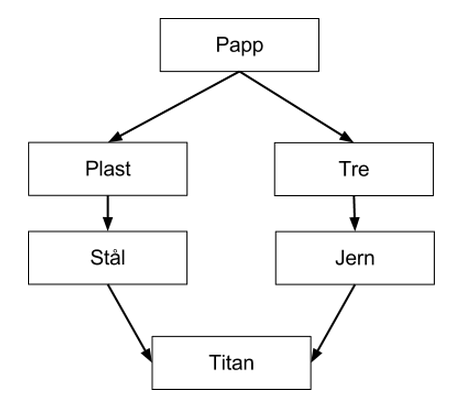
\includegraphics[scale=0.5]{images/oppgraderingstre}
	\end{center}
	\caption{Ressursoppgraderinger}
\end{figure}

\subsubsection{Ressursutvinning}
Spillere skaffer seg ressurser ved å gjenvinne søppel som ligger
spredt rundt på øya. Dette blir gjort ved hjelp av miljøstasjonen
som hver spiller starter med. For å aktivisere spilleren må en "fysisk" dra søppel fra øya og over på miljøstasjonen. Denne vil så bruke noe tid på å prosessere søplet og gjenvinne ressurser fra dette.


\subsubsection{Miljøstasjon} \label{miljostasjon}
Miljøstasjonen er det mest sentrale spillelementet i Garbage
Alert. Denne kan bli sett på som hovedbasen i spillet.
Miljøstasjonen kan oppgraderes på tre måter for å forbedre effektiviteten:

\begin{description}
	\item \textbf{Volum/Utvinningsgrad}\\
		Denne oppgraderingen kan øke utvinningsgraden og volumet av søppel som blir brukt i gjennvinningsprosessen. Restavfallet (søppelet som ikke blir gjenvunnet) vil på magisk vis bli borte. Tabell \ref{tab:effektivitet} viser oppgraderingene for Volum/Utvinningsgrad. Man starter på nivå 0, og deretter kan man oppgradere ett trinn ad gangen.
	\item \textbf{Buffer}\\
		Miljøstasjonen kan få en buffer hvor spilleren kan samle opp søppel, som automatiserer gjenvinningsprosessen til en viss grad. Dermed kan spilleren bruke mindre tid på å sørge for at søppelet på øya blir flyttet til miljøstasjonen.
	\item \textbf{Ressurser}\\
		For å kunne gjenvinne nye typer ressurser må spilleren oppgradere miljøstasjonen. Her får spilleren valget mellom to ulike veier som vil avgjøre hvilke ressurser spilleren får tilgang til (se figur \ref{fig:ressursoppgraderinger}).
\end{description}

\begin{table}
	\begin{tabular}[\textwidth]{ l  l  p{3cm}  l  p{4cm} }
		\hline
		\bf{Effektivitet} & \bf{Utvinningsgrad} & \bf{Volum} & \bf{Tid} & \bf{Ressurskrav} \\
		\hline
		Nivå 0 & 10 & 10 & 15sek & Ingen  \\
		Nivå 1 & 20 & 10 & 15sek & Papp \\
		Nivå 2 & 30 & 10 & 15sek & Papp, og plast eller tre \\
		Nivå 3 & 30 & 20 & 15sek & Papp, plast, tre, stål, jern og titan \\
		\hline
	\end{tabular}
	\label{tab:effektivitet}
	\caption{Oppgraderinger for Volum/Utvinningsgrad}
\end{table}


\subsubsection{Angrep}
En spiller får utdelt tre angrepsplattformer. På disse tre plattformene
kan spilleren velge hvilke angrep han vil utvikle, basert på hvilke
tilgjengelige ressurser han har. Når en spiller bygger et våpen kan dette avfyres et bestemt antall ganger med en buffertid imellom skuddene. Erfaringer fra alfa-testing av spillet viste at tre skudd med en buffertid på 30 sekunder var passende. Når våpenets ammunisjon er brukt opp må man kjøpe et nytt våpen for å fortsette sine angrep. 

I tillegg til å avfyre skudd må spilleren sørge for at det er søppel på angrepsplattformen, ettersom målet med et angrep ikke bare er å skade motspillerenes bygninger, men også bli kvitt søppel. Hvis den forsvarende motspilleren ikke har mur, eller muren blir ødelagt i angrepet vil det avfyrte søppelet lande på motspillerens øy.

Rekkefølgen for hva som blir skadet under ett angrep er: forsvar, angrep, miljøstasjon. Det vil si at dersom man ikke har mur, eller muren blir ødelagt under angrepet, vil våpenene til spilleren ta skade. Dersom spilleren verken har mur eller våpen vil miljøstasjonen ta skade under et angrep. 


\subsubsection{Forsvar}
Spillere kan bygge forsvar rundt øya si. Dette forsvaret vil forhindre at motspillere skader ens våpen og miljøstasjon. Det finnes ulike typer forsvarsmurer, som er tilgjengelige i tråd med hvilke ressursoppgraderinger man har. 


\subsubsection{Oppgraderinger av forsvar og angrep}
En spiller som har en type mur, kan oppgradere muren til en bedre mur. En slik oppgradering er billigere enn å bygge en ny mur. Ideen bak dette er at materialene den gamle muren består av blir brukt til å bygge den nye muren, i tillegg til ekstra materialer som kreves i henhold til oppgraderingen. Tilsvarende kan gjøres for våpen.


\subsubsection{Reparasjoner}
Både mur, våpen og miljøstasjon kan repareres. Prisen på en reparasjon tar et prosentvis utgangspunkt i prisen på en ny bygning. I tillegg antas det at 50\% av den ødelagte delen av bygningen kan gjenbrukes. Eksempelvis så kan en mur som har mistet halvparten av hitpointsene sine repareres for 25\% av prisen på en ny mur (halvparten av de ødelagte materialene kan brukes igjen, dermed må spilleren kun betale for den resterende fjerdedelen av muren).


\subsubsection{Priser, helsepoeng og angrepsverdier}
Under utviklingen og alfa-testingen av spillet har Re3 kommet frem til en prisliste, helsepoeng på våpen, mur og miljøstasjon samt attack-verdier for våpnene.

Prislisten er utviklet slik at det hele tiden er knapt med ressurser. Det vil si at nesten alle bygninger og oppgraderinger koster noe papp, osv, for at denne ressursen ikke hoper seg opp. Utkastet av prislisten finnes i appendiks \ref{A}.

Tanken bak helsepoengene og angrepsverdiene er at to angrep av et type våpen ødelegger en mur bygget av samme ressurs som våpenet. Det vil si at to angrep fra en katapult ødelegger en tremur. Et våpen som er et nivå høyere enn forsvaret vil ødelegge 90\% av muren. Dersom angrepet er to nivå (eller mer) høyere enn forsvaret vil muren bli ødelagt i tillegg til at våpen/miljøstasjon vil ta skade. Et komplett utkast over helsepoeng og angrepsverdier finnes i appendiks \ref{B}. Disse verdiene er dog det mest usikre med denne prototypen, og er noe som må justeres gjennom mye utprøving.

